% Copyright 2021 Edoardo Riggio

% Licensed under the Apache License, Version 2.0 (the "License");
% you may not use this file except in compliance with the License.
% You may obtain a copy of the License at

% 	http://www.apache.org/licenses/LICENSE-2.0

% Unless required by applicable law or agreed to in writing, software
% distributed under the License is distributed on an "AS IS" BASIS,
% WITHOUT WARRANTIES OR CONDITIONS OF ANY KIND, either express or implied.
% See the License for the specific language governing permissions and
% limitations under the License.

\documentclass{article}

\usepackage{hyperref, amsmath, graphicx, amssymb}
\usepackage{fancyvrb,newverbs,xcolor}

\graphicspath{ {./assets/} }

\definecolor{cverbbg}{gray}{0.93}

\newenvironment{cverbatim}
 {\SaveVerbatim{cverb}}
 {\endSaveVerbatim
  \flushleft\fboxrule=0pt\fboxsep=.5em
  \colorbox{cverbbg}{\BUseVerbatim{cverb}}%
  \endflushleft
}

\newenvironment{lcverbatim}
 {\SaveVerbatim{cverb}}
 {\endSaveVerbatim
  \flushleft\fboxrule=0pt\fboxsep=.5em
  \colorbox{cverbbg}{%
    \makebox[\dimexpr\linewidth-2\fboxsep][l]{\BUseVerbatim{cverb}}%
  }
  \endflushleft
}

\newcommand{\ctexttt}[1]{\colorbox{cverbbg}{\texttt{#1}}}
\newverbcommand{\cverb}
  {\setbox\verbbox\hbox\bgroup}
  {\egroup\colorbox{cverbbg}{\box\verbbox}}

\begin{document}
\begin{titlepage}
    \begin{center}
        \vspace*{1cm}
        
        \Huge
        \textbf{Information Retrieval Cheatsheet}
        
        \vspace{0.5cm}
        \LARGE
        
        \vspace{.5cm}
        
        Edoardo Riggio
   		  \vspace{1.5cm}
       
        \vfill
        
        \today
        
        \vspace{.8cm}
          \Large
          Information Retrieval - S.A. 2021 \\
        Computer Science\\
        Universit\`{a} della Svizzera Italiana, Lugano\\
        
    \end{center}
\end{titlepage}

\tableofcontents

\newpage

\section{Introduction}
\subsection{Text Information Systems}
Text Information Systems involve three main capabilities:

\begin{itemize}
	\item \textbf{Text Retrieval}
	\vspace{.2cm} \\
	Information Retrieval is a field concerned with the structure, analysis, organization, storage searching, and retrieval of information.
	
	\item \textbf{Text Analysis}
	\vspace{.2cm} \\
	Analyze large amounts of text data in order to discover interesting patterns buried in text.
	
	\item \textbf{Text Organization}
	\vspace{.2cm} \\
	Annotate a collection of text documents with meaningful topical structures so that scattered information can be connected and navigated.
\end{itemize}
While text retrieval is part of information retrieval, text analysis and text organization are part of text mining. \\ \\
Differently from queries done on DBMS, queries in search engines make use of natural language. It is much harder to compare the text query to the document text and determining what is a good match and what is not a good match. This is the core issue of information retrieval. There are many different ways of writing the same thing, thus an identical matching of words is not enough.

\subsection{Relevance}
A document is said to be relevant when it contains the information that a person was looking for when he/she submitted the query tot eh search engine.\\ \\
In order to understand what the user is asking for in the query, we use something that is known as \textbf{NLP} (Natural Language Processing). NLP is concerned with developing techniques for enabling computers to understand the meaning of natural language text.

\section{Text Access}
Text data access is the foundation for text analysis. The general goal of text data access is to connect users with the right information at the right time. \\ \\
Connection with users can be done in two ways:

\begin{itemize}
	\item \textbf{Pull}
	\vspace{.2cm} \\
	The user takes initiative in order to fetch relevant information from the system.
	
	\item \textbf{Push}
	\vspace{.2cm} \\
	The system takes initiative in order to offer relevant pieces of information to the users.
\end{itemize}

\subsection{Access Mode: Pull vs Push}
In \textbf{pull} mode, the user initiates the access process in order to find the relevant text data. When a user has such need, then this can be done in two different ways:

\begin{itemize}
	\item \textbf{Querying}
	\vspace{.2cm} \\
	The user can use a query in order to obtain ad hoc information. This mode of research is done by using a few -- yet specific -- words.
	
	\item \textbf{Browsing}
	\vspace{.2cm} \\
	It is a way of accessing text data, and can be very useful for users when they do not know how to formulate an effective query.
\end{itemize}
In \textbf{push} mode, the system initiates the process to recommend a set of relevant information items to the user. \\ \\
Broadly, there are two kinds of information needs:

\begin{itemize}
	\item \textbf{Short-Term Needs}
	\vspace{.2cm} \\
	These needs are often associated with pull mode. This type of information need is temporary and usually satisfied through searching or browsing.
	
	\item \textbf{Long-Term Needs}
	\vspace{.2cm} \\
	These needs are often associated will pull mode. This type of information need can be better satisfied through filtering or recommendation of the system to the user.
\end{itemize}
Finally we have \textbf{browsing traces}. These traces happen whenever a user does any kind of browsing. They are used in order to model the behaviour of the user, and make more precise recommendations.

\subsection{Search Engine Architecture}
A \textbf{software architecture} consists of software components, the interfaces provided by those components, and the relationships between them. \\ \\
The software architecture of a search engine is determined by the following requirements:

\begin{itemize}
	\item \textbf{Effectiveness}
	\item \textbf{Efficiency}
\end{itemize}
An information retrieval process can be divided into four subprocesses:

\begin{enumerate}
	\item \textbf{Indexing Process}
	\vspace{.2cm} \\
	This process is composed of several different stages. First we have \textbf{text acquisition}, in which the system identifies and stores documents for indexing. \\ \\
	Second we have \textbf{text transformation}, in which the system transforms documents into index terms or features. \\ \\
	Finally we have \textbf{index creation}, in which the system takes index terms and creates data structures to support fast searching.
	
	\item \textbf{Query and Retrieval Process}
	\vspace{.2cm} \\
	It is composed of the following stages. \textbf{User interaction}, which supports the creation of a query and displays the results. \\ \\
	Next we have \textbf{ranking and retrieval}, in which the query and indices are used in order to generate a ranked list of documents. \\ \\
	Finally we have \textbf{evaluation}, which monitors and measures the effectiveness and efficiency of the information retrieval system.
	
	\item \textbf{Relevance Feedback Process}
	\vspace{.2cm} \\
	It is composed of three parts. The first part is the \textbf{user evaluation}, where the user assesses the effectiveness of the system. \\ 
	Then we have \textbf{user feedback}, which supports refinement of the query and display of the result.\\
	Finally we have \textbf{ranking and retrieval}, where the system generates a ranked list of the documents.
\end{enumerate}

\subsection{Formal Definition of Information Retrieval}
Information retrieval is composed of several elements, such as:

\begin{itemize}
	\item \textbf{Vocabulary}
	\vspace{.2cm} \\
	Vocabulary is defined as:
	\[ V = \{ w_1, w_2, ..., w_n \} \]
	This represents the vocabulary of a language.
	
	\item \textbf{Document}
	\vspace{.2cm} \\
	A document is defined as:
	\[ d_i = d_{i1}, ..., d_{iM} \]
	Where $d_{ij} \in V$.
	
	\item \textbf{Collection}
	\vspace{.2cm} \\
	A collection is defined as:
	\[ C = \{d_1, ..., d_M\} \]
	this represents a collection of documents.
	
	\item \textbf{Query}
	\vspace{.2cm} \\
	A query is defined as:
	\[ q = q_1, ..., q_M \]
	Where $q_j \in V$.
	
	\item \textbf{Relevant Documents}
	\vspace{.2cm} \\
	This set is defined as:
	\[ R(q) \subseteq C \]
	And it is generally unknown and user-dependent. The query acts as a hint on which the document must be contained in $R(q)$.
\end{itemize}

\subsection{How to Compute $R'(q)$}
$R'(q)$ can be computed in one of two ways:

\begin{itemize}
	\item \textbf{Document Selection}
	\vspace{.2cm} \\
	This can be described as:
	\[ R'(q) = \{ d \in C~|~f(d, q) = 1 \} \]
	Where $f(d, q) \in \{0,1\}$ and is an indicator function/binary classifier. Here the system must decide whether a document is relevant or not -- i.e. \textbf{absolute relevance}. This is also known as \textbf{boolean retrieval}.
	
	\item \textbf{Document Ranking}
	\vspace{.2cm} \\	
	This can be defined as:
	\[ R'(q) = \{ d \in C~|~f(d,q) > \Theta\} \]
	Where $f(d,q) \in \mathbb{R}$ is a relevance measure function, and $\Theta$ is a cutoff determined by the user. Here the system only decides if one document is more likely relevant than another -- i.e. \textbf{relative measure}. This is also known as \textbf{ranked retrieval}.
\end{itemize}

\section{Implementation of an IR System}
An information retrieval system is mainly made up of four components:

\begin{enumerate}
	\item \textbf{Tokenizer}
	\vspace{.2cm} \\
	This component takes in documents as raw strings and determines how to separate the large document into separate tokens.
	
	\item \textbf{Indexer}
	\vspace{.2cm} \\
	This module processes documents and indexes them with appropriate data structures. This module can be ran offline.
	
	\item \textbf{Scorer/Ranker}
	\vspace{.2cm} \\
	This module takes a query and returns a ranked list of documents.
\end{enumerate}

\subsection{Indexing}
The main role of the indexer is to convert documents into data structures in order to enable fast search. The \textbf{inverted index} is the dominant indexing method for supporting basic search algorithms. \\ \\
This data structure is composed of two parts:

\begin{itemize}
    \item \textbf{Lexicon}
	\vspace{.2cm} \\
	It is a table of search-specific information, such as document frequency and where to find in the postings the per-document term counts
	
	\item \textbf{Posting File}
	\vspace{.2cm} \\
	It is a mapping that goes from any term integer ID to a list of documents IDs and frequency information of the term in those documents.
\end{itemize}
Before obtaining the inverted index we need to pre-process the documents in order to extract only the features we are interested in.

\subsection{Zipf's Law}
The distribution of words in documents is very skewed. This means that only a few words occur often, while many other words occur rarely. \\ \\
Zipf's Law says that the rank $r$ of a word times its frequency $f$, is approximately a constant $k$ -- assuming that the words are ranked in decreasing order of frequency. Thus we have the following formula:
\[ r \cdot f \approx k \] \\
In the following case, for example, the words on the far right -- with $x = [0, 7.5)$ -- are high frequency words, thus useless, the words in the middle -- with $x = [7.5, 15)$ -- are intermediate frequency words, thus very useful, and the words in the far right -- with $x = [15,25]$ -- are rare words, thus they might be useful. \\ \\

\begin{center}
	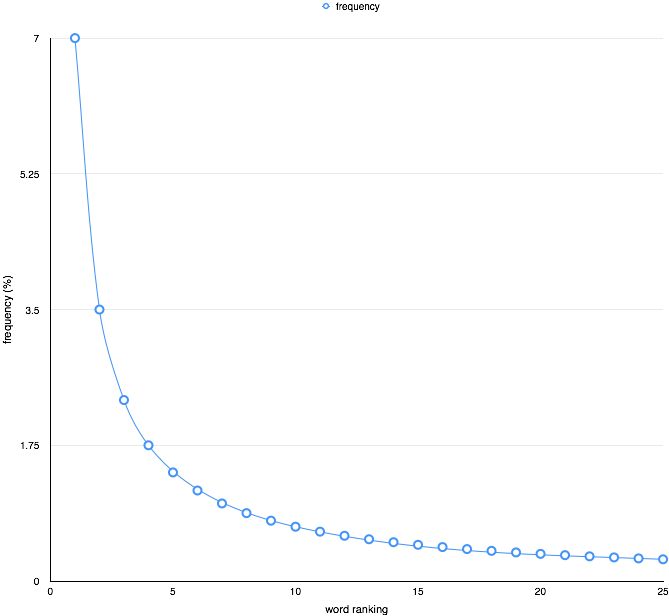
\includegraphics[width=7cm]{zipf.png}
\end{center}

\subsection{Text Indexing}
Text indexing can be divided into the following steps:

\begin{enumerate}
	\item \textbf{Tokenization}
	\item \textbf{Stopword Removal}
	\item \textbf{Stemming}
	\item \textbf{Detecting Phrases}
	\item \textbf{POS Tagging and N-Grams}
	\item \textbf{Processing Document Structure and Markup}
	\item \textbf{Named Entity Recognition}
	\item \textbf{Link Analysis}
	\item \textbf{Build the Inverted Index}
	\item \textbf{Compress the Inverted Index}
\end{enumerate}

\subsubsection{Tokenizing}
To tokenize means to break down words into appropriate sequences of characters. \\ \\
The first step is to use the \textbf{parser} in order to identify the appropriate parts of the document that need to be tokenized.

\subsubsection{Stopping Removal}
Some words have little to no meaning on their own and occur very frequently. These are treated as stopwords and removed. Although, sometimes, they could be important in combination with other words.

\subsubsection{Stemming}
Many morphological variations of words exist. In most cases, these have the same or very similar meanings. The goal of \textbf{stemmers} is to attempt to reduce morphological variations of words to a common stem. \\ \\
For example, the words \textit{consign}, \textit{consigned}, \textit{consigning} and \textit{consignment} can all be reduced down to \textbf{consign}. \\ \\
There are two main types of stemming approaches:

\begin{itemize}
	\item \textbf{Algorithmic Approach}
	\vspace{.2cm} \\
	In this case it is a program that determines related words. This could give some false positives and many false negatives.
	
	\item \textbf{Dictionary-Based Approach}
	\vspace{.2cm} \\
	In this case a list of related words is used. Endings are removed based on a dictionary. This approach produces real words, not stems, and it's much more precise -- but more expensive to run.
\end{itemize}
Some used stemmers are:

\begin{itemize}
	\item \textbf{Porter Stemmer}
	\vspace{.2cm} \\
	This is an algorithm used since the 70s. It consists of a series of rules designed to remove the longest possible suffix from a word at each step. It produces stems, not real words. Sometimes this algorithm can be too aggressive or too weak. Porter2 stemmer was created in order to address some of the issues Porter had.
	
	\item \textbf{Krovertz Stemmer}
	\vspace{.2cm} \\
	This is a hybrid algorithmic-dictionary stemmer. The word is checked in a dictionary. If the word is present, then the word is either left alone or replaced with "exception", if the word is not present, the word is checked for suffixes that could be removed. Finally, after the removal, the dictionary is checked again. \\ \\
	In this case words are generated, not stems. Furthermore, this stemmer has lower false positives, but higher false negatives.
\end{itemize}

\subsubsection{POS Tagger and N-Grams}
\textbf{POS (Part Of Speech) tagging} is the process of marking up a word in a text as corresponding to a particular part of speech, based on both its definition and its context. POS taggers use statistical models of text in order to predict syntactic tags of words. \\ \\
Since POS tagging is too slow for some collections, \textbf{N-Grams} also exist. These are typically formed from overlapping sequences of words. Frequent N-Grams are more likely to be useful phrases. N-Grams follow Zipf's distribution.

\subsubsection{Build the Inverted Index}
In order to construct an inverted index, we use sort-based methods by following these steps:

\begin{enumerate}
	\item Collect local tuples, such as term IDs, Doc IDs and frequency;
	\item Sort the local tuples;
	\item Perform pair-wise merge runs;
	\item Output the inverted file.
\end{enumerate}
While the dictionary part of the inverted index is of modest size, the postings part is huge and stored on disk.

\subsection{Ranking Documents}
The formula that is used in order to rank documents is the following.
\[ f(q, d) = f_a (h (g (t_1, d, q), ..., g (t_k, d, q)), f_d(d), f_q(q)) \]
Where $f_d(q)$ and $f_q(q)$ are pre-computed. Moreover, a score accumulator is maintained for each $d$ in order to compute $h$. Finally, for each query term $t_i$, the following inverted list is fetched.
\[ \{ (d_1, f_1), ..., (d_n, f_n) \} \]
In order to improve the efficiency of the ranker, one could use caching, and keep only the most promising accumulators. There is no need for parallel processing.

\section{Retrieval Models}
The retrieval process is based on a retrieval model which matches a query with a document. There are at least two classes of retrieval models:

\begin{itemize}
	\item \textbf{Set-Based Models}
	\vspace{.2cm} \\
	These are models like the Boolean model, and are defined by the following function:
	\[ f(q, d) = \{ 0,1 \} \]
	
	\item \textbf{Similarity-Based Models}
	\vspace{.2cm} \\
	These are models such as the vector space model, the probabilistic model... They are defined by the following function:
	\[ f(q,d) = \text{similarity}(q, d) = [0, \infty) \]
\end{itemize}

\subsection{Examples of Retrieval Models}
\subsubsection{Boolean Model}
A boolean model can only have two possible outcomes for query processing: true or false. It is an exact-match retrieval process, and the simplest for of ranking. \\ \\
A query is usually specified using boolean operators (such as AND, NOT, OR...), and is used in DBMSs. \\ \\
Some advantages of boolean retrieval are:

\begin{itemize}
	\item The result is predictable;
	\item Many different features can be incorporated;
	\item Efficient query processing.
\end{itemize}
While the disadvantages are:

\begin{itemize}
	\item The effectiveness of the query solely depends on the user;
	\item Simple queries do not usually work well;
	\item Complex queries are difficult both to think and to write.
\end{itemize}

\subsubsection{Ranked Retrieval}
In ranked retrieval, documents are presented according to how much they match the query. In a good ranking function relevant documents should be ranked on top of non-relevant ones.

\subsection{Designing Retrieval Models}
All retrieval models are based on the assumption of using a \textbf{bag-of-words} representation of text. A bag-of-words is a model in which a text is represented as the multiset of its words, disregarding grammar and even word order. \\ \\
In order to design a retrieval function, we require a computational definition of relevance. Moreover, we need to use features such as:

\begin{itemize}
	\item \textbf{Term Frequency (TF)}
	\vspace{.2cm} \\
	This represents how many times does one term appear inside of each document.
	
	\item \textbf{Document Length}
	\vspace{.2cm} \\
	If a term occurs in a long document many times, it is not as significant as a term that occurs the same number of times inside a short document.
	
	\item \textbf{Document Frequency (DF)}
	\vspace{.2cm} \\
	This represents how often a term appears at least once in any document of the entire collection.
\end{itemize}

\subsection{Vector Space Model}
This is a simple, yet effective, way of designing ranking functions for information retrieval systems. This is a special case of similarity-based models, where we assume that relevance is roughly correlated to the similarity between a query and a document. \\ \\
In this representation, each dimension of a highly dimensional space represents a term. We can plot the documents in the collection as vectors of term magnitude.

\begin{center}
	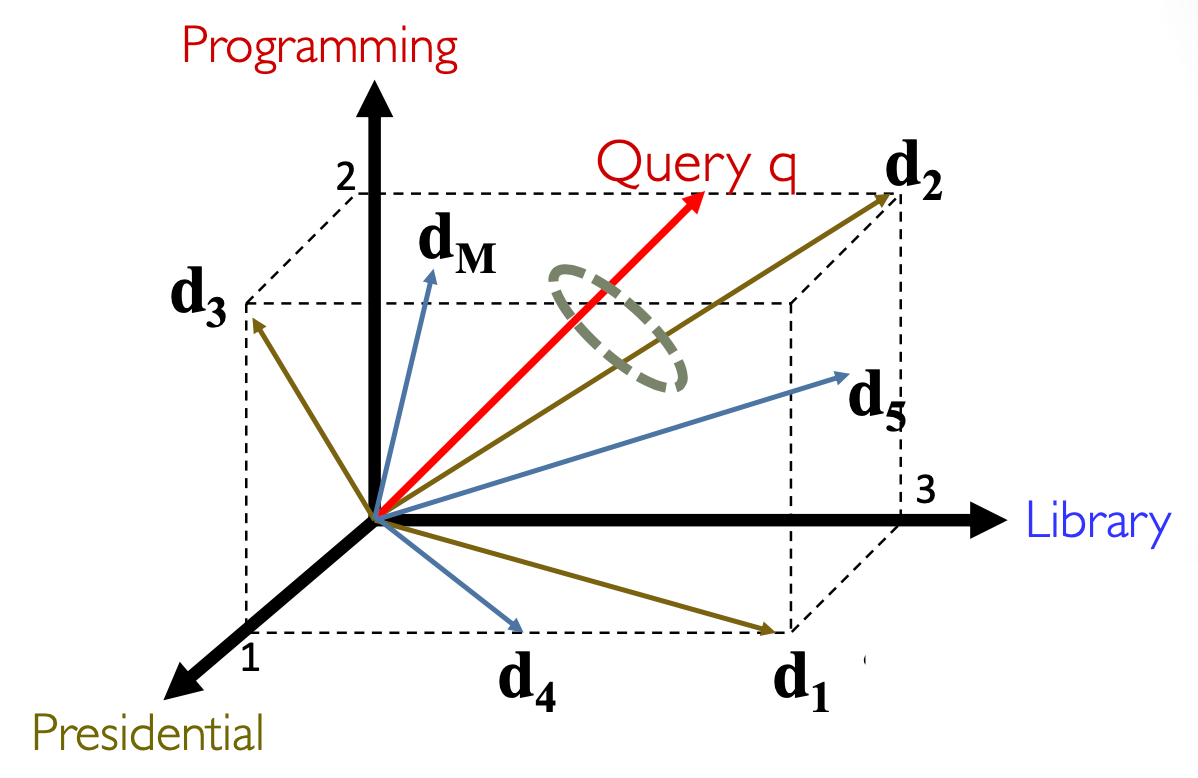
\includegraphics[width=9cm]{vsm.png}
\end{center}
This is a framework, thus it needs to be defined. In order to use this framework we need the following:

\begin{itemize}
	\item \textbf{Dimension Instantiation}
	\vspace{.2cm} \\
	The number of dimension can be defined by the number of words inside of a bag-of-words.
	
	\item \textbf{Vector Placement}
	\vspace{.2cm} \\
	In order to place the vector inside of the framework, we can use bit vectors. These bit vectors can only be either 0 or 1. We will have a 1 if the word $w_i$ -- one of the words of the axes -- is present in the document or query, 0 otherwise.
	
	\item \textbf{Similarity Instantiation}
	\vspace{.2cm} \\
	The similarity between a query and a document can be defined as the dot product between these two vectors. In this case the formula would be:
	\[ \text{sim}(q, d) = \langle q, d \rangle = \sum^N_{i = 1} x_i \cdot y_i \]
\end{itemize}
By using only these definitions and instantiations, the framework will be limited. For example, wouldn't it be correct to give more credit to terms that appear more times in a document or query? The current model does not allow it. This is why we can introduce some improvements to the current model, such as:

\begin{itemize}	
	\item \textbf{Term Frequency Vector}
	\vspace{.2cm} \\
	An improvement can be applied by representing a frequency vector. This vector will represent the number of times that the word $w_i$ -- one of the words of the axes -- is contained in the query or in the document.
	
	\item \textbf{Term Frequency Weighting (TFW)}
	\vspace{.2cm} \\
	This improvement consists in using the same formula as the one used in the similarity instantiation, but with $q$ and $d$ represented by term frequency vectors.
	
	\item \textbf{Inverse Document Frequency}
	\vspace{.2cm} \\
	This improvement consists in giving a weight to words. The formula for computing $y_i$ is given by:
	\[ y_i = \text{count}(w_i, q) * \log \left( \frac{M+1}{k} \right) \]
	Where $\text{count}(w_i, q)$ is the number of times the word $w_i$ appears in document $d$, $M$ is the total number of documents in a collection, and $k$ is the total number of documents containing the word $w$. \\ \\
	The weight of each word inside of the collection of documents is computed by the second part of the previous formula, i.e.
	\[ \log \left( \frac{M+1}{k} \right) \]
\end{itemize}

\subsubsection{TF Transformation}
Since the inverse document frequency still has some problems, we can use TF transformation in order to normalize the number of times a word appears in a collection. This method is used in order to avoid the dominance of a single term above all the others. \\ \\
This transformation, is mathematically defined as follows:

\[ f(q, d) = \sum_{w \in q \cap d} \text{count}(w, q) \cdot \frac{(k+1) \cdot \text{count}(w, d)}{\text{count}(w, d) + k} \cdot \log \left( \frac{M+1}{df(w)} \right) \]
Where $k \geq 0$ is a constant, $w \in q \cap d$ indicates all matched query words in the document, and $df(w)$ indicates the document frequency of the word $w$.

\subsubsection{Document Length Normalization}
Since a long document has a higher chance of matching any query, it must be penalised -- but not too much -- by using a document length normalizer. In order to not over-penalise a long document, we say that a document with more words must be penalised more, while a document with more contents must be penalised less. \\ \\
In order to normalize the document lengths, we use the average document length as a pivot. The formula of the document length normalizer is the following:
\[ 1 - b + b \cdot \left( \frac{|d|}{\text{avgdl}} \right) \]
Where $b \in [0, 1]$ is a constant and \textit{avgdl} is the average length of the documents in the collection.

\subsection{Probabilistic Models}
In probabilistic models, we define the ranking function based on the probability that a given document $d$ is relevant to a query $q$.
\[ p(R = 1~|~d,q) \]
Where $R \in \{ 0,1 \}$ is a binary random variable that denotes relevance. In order to define relevance in a model such as this, we use the following formula.
\[ p(R=1~|~q,d) = \frac{\text{count}(R=1, d,q)}{\text{count}(d,q)} \]

\subsection{Query Likelihood Retrieval Model}
In query likelihood models, our assumption is that the probability of relevance can be approximated by the probability of a query given a document and a relevance.
\[ p(q~|~d, R=1) \]
This captures the following probability: if a user likes document $d$, how likely would the user enter query $q$ in order to retrieve document $d$? In this model we assume that the user imagines some ideal document, and generates a query based on that ideal document.

\subsection{Statistical Language Model}
A statistical language model is used in order to compute the probability of text. For example:

\begin{align*}
	p(\text{\textit{"Today is Wednesday"}}) & \approx 0.001 \\
	p(\text{\textit{"Today Wednesday is"}}) & \approx 0.0000000000001 \\
	p(\text{\textit{"The eigenvalue is positive"}}) & \approx 0.00001
\end{align*} \\
This probability distribution over word sequences is highly context- and user-dependent. This is also called a generative model. \\ \\
Language model is useful to quantify the uncertainties in natural language. It can be particularly useful in:

\begin{itemize}
	\item \textbf{Speech Recognition}
	\item \textbf{Text Categorization}
	\item \textbf{Information Retrieval}
\end{itemize}

\subsubsection{Unigram Language Model}
Unigram language model is the simplest form of a language model. It generates text by generating each word independently. Thus:
\[ p(w_1, w_2, ..., w_n) = p(w_1) + p(w_2) + ... + p(w_n) \]
In order to compute a more accurate estimation of unigrams, we could use topic representation. To do so we get:

\begin{itemize}
	\item \textbf{Background Language Model}
	\vspace{.2cm} \\
	This LM is composed of terms contained in a general background English text. Mathematically this is equal to:
	\[ p(w~|~B) \]
	
	\item \textbf{Topic Language Model}
	\vspace{.2cm} \\
	This LM is composed of terms contained in a collection based on a topic -- for example all words that appear in computer science papers. Mathematically this is equal to:
	\[ p(w~|~C) \]
\end{itemize}
Given these two LMs, we can compute a normalized LM which can then be used with the original text. The normalized LM is given by:
\[ \frac{p(w~|~T)}{p(w~|~B)} \]

\subsubsection{Query Generation}
We can consider $p(q~|~d)$ to be made up of independent terms. This way the probability becomes a product of the probabilities of of each query word in each document's language model. In order to formally state this, we consider a query $q$ that contains the words:
\[ q = w_1, w_2, ..., w_n \]
Such that $|q| = n$. The scoring or ranking function will thus be:
\[ p(q~|~d) = p(w_1~|~d) \cdot p(w_2~|~d) \cdot ... \cdot p(w_n~|~d) \]
In practice, we score the document for this query by using the logarithm of the query likelihood.

\begin{align*}
	\text{score}(q,d) & = \log p(q~|~d) \\
	& = \sum^{n}_{i=1} \log p(w_i~|~d) \\
	& = \sum_{w \in V} \text{count}(w, q) \cdot \log p(w~|~d)
\end{align*}
Where $V$ is the vocabulary.

\subsubsection{Smoothing the Document LM}
In order to estimate the $p(w~|~d)$ in the formula above, we can use the MLE (Maximum Likelihood Estimator). This will make sure that the curve given by $p(w~|~d)$ is smoother.
\[ p_{ML}(w~|~d) = \frac{\text{count}(w, d)}{|d|} \]
Now $p(w~|~d)$ will be always positive, even if $\text{\textit{count}}(w, d) = 0$. Now, we also need to consider what probability should be assigned to unseen words. This is the equation used in order to smooth the curve:
\[ p(w~|~d) = \begin{cases} p_{\text{\textit{seen}}}(w~|~d) & \text{if \textit{w} is seen in \textit{d}} \\ \alpha_d \cdot p(w~|~C) & \text{otherwise} \end{cases} \]
Where $p_{\text{\textit{seen}}}(w~|~d)$ is the discounted MLE, and $C$ is the collection language model. Finally we can rewrite the ranking function accounting for smoothing. The components of the new function are the following:

\begin{itemize}
	\item \textbf{Query Words Matched in \textit{d}}
	\vspace{.2cm} \\
	The formula is:
	\[ \sum_{w \in V,~\text{count}(w, d) > 0} \text{count}(w, q) \cdot \log(p_{\text{\textit{seen}}}(w~|~d)) \]
	
	\item \textbf{Query Words not Matched in \textit{d}}
	\vspace{.2cm} \\
	The formula is:
	\[ \sum_{w \in V,~\text{count}(w, d) = 0} \text{count}(w,q) \cdot \log (\alpha_d \cdot p(w~|~C)) \]
	
	\item \textbf{All Query Words}
	\vspace{.2cm} \\
	The formula is:
	\[ \sum_{w \in V} \text{count}(w, q) \cdot \log (\alpha_d \cdot p(w~|~C)) \]
\end{itemize}
An the final equation will be:
\begin{align*}
	\text{score}(q,d)  = & \sum_{w \in V} \text{count}(w, q) \cdot \log p(w~|~d) \\
	= & \sum_{w \in V,~\text{count}(w, d) > 0} \text{count}(w, q) \cdot \log(p_{\text{\textit{seen}}}(w~|~d)) \\
	& + \sum_{w \in V,~\text{count}(w, d) = 0} \text{count}(w,q) \cdot \log (\alpha_d \cdot p(w~|~C)) \\
	= & \sum_{w \in V} \text{count}(w, q) \cdot \log (\alpha_d \cdot p(w~|~C)) \\
	& - \sum_{w \in V,~\text{count}(w, d) > 0} \text{count}(w, q) \cdot \log (\alpha_d \cdot p(w~|~C)) \\
	= & \sum_{\substack{w \in d \\ w \in q}} \text{count}(w,q) \cdot \log \left( \frac{p_\text{\textit{seen}}(w~|~d)}{\alpha_d \cdot p(w~|~C)} \right) + n \log (\alpha_d) + \sum_{w \in V} \log(p(w~|~C))
\end{align*}
By rewriting the formula, the following features are now incorporated in the ranking function:

\begin{itemize}
	\item \textbf{Matched Query Terms}
	\vspace{.2cm} \\
	This can be seen in:
	\[  \sum_{\substack{w \in d \\ w \in q}} ... \]
	
	\item \textbf{TF Weighting}
	\vspace{.2cm} \\
	This can be seen in:
	\[ p_\text{\textit{seen}}(w~|~d) \]
	
	\item \textbf{IDF Weighting}
	\vspace{.2cm} \\
	This can be seen in:
	\[ \alpha_d \cdot p(w~|~C) \]
	
	\item \textbf{Document Length Normalization}
	\vspace{.2cm} \\
	This can be seen in:
	\[ n \log (\alpha_d) \]
\end{itemize}
Other smoothing methods can be used, two of the main ones are:

\begin{itemize}
	\item \textbf{Linear Interpolation Smoothing}
	\vspace{.2cm} \\ 
	Which is also known as Jelinek-Mercer Smoothing.
	
	\item \textbf{Bayesian Smoothing}
	\vspace{.2cm} \\
	Which is also known as Dirichlet Prior Smoothing
\end{itemize}

\section{Feedback Models}
There are three major forms of feedback:

\begin{itemize}
	\item \textbf{Relevance Feedback}
	\vspace{.2cm} \\
	The user expressively indicates the documents that are relevant to the query.
	
	\item \textbf{Pseudo Feedback}
	\vspace{.2cm} \\
	The system assumes the top retrieved documents as relevant.
	
	\item \textbf{Implicit Feedback}
	\vspace{.2cm} \\
	The system monitors what the user does and based on that it makes some assumptions on the document relevance.
\end{itemize}

\subsection{Relevance Feedback}
The user can make judgements about whether each returned document is useful or not. With relevance feedback we can perform two operations on the query:

\begin{itemize}
	\item \textbf{Query Expansion}
	\vspace{.2cm} \\
	It is when new weighted terms are added.
	
	\item \textbf{Query Modification}
	\vspace{.2cm} \\
	It is when the weights of existing terms are adjusted.
\end{itemize}

\subsection{Rocchio Feedback}
The Rocchio Feedback is a relevance feedback algorithm applied to the VSM (Vector Space Model). The following is a representation of the Rocchio Feedback.

\begin{center}
	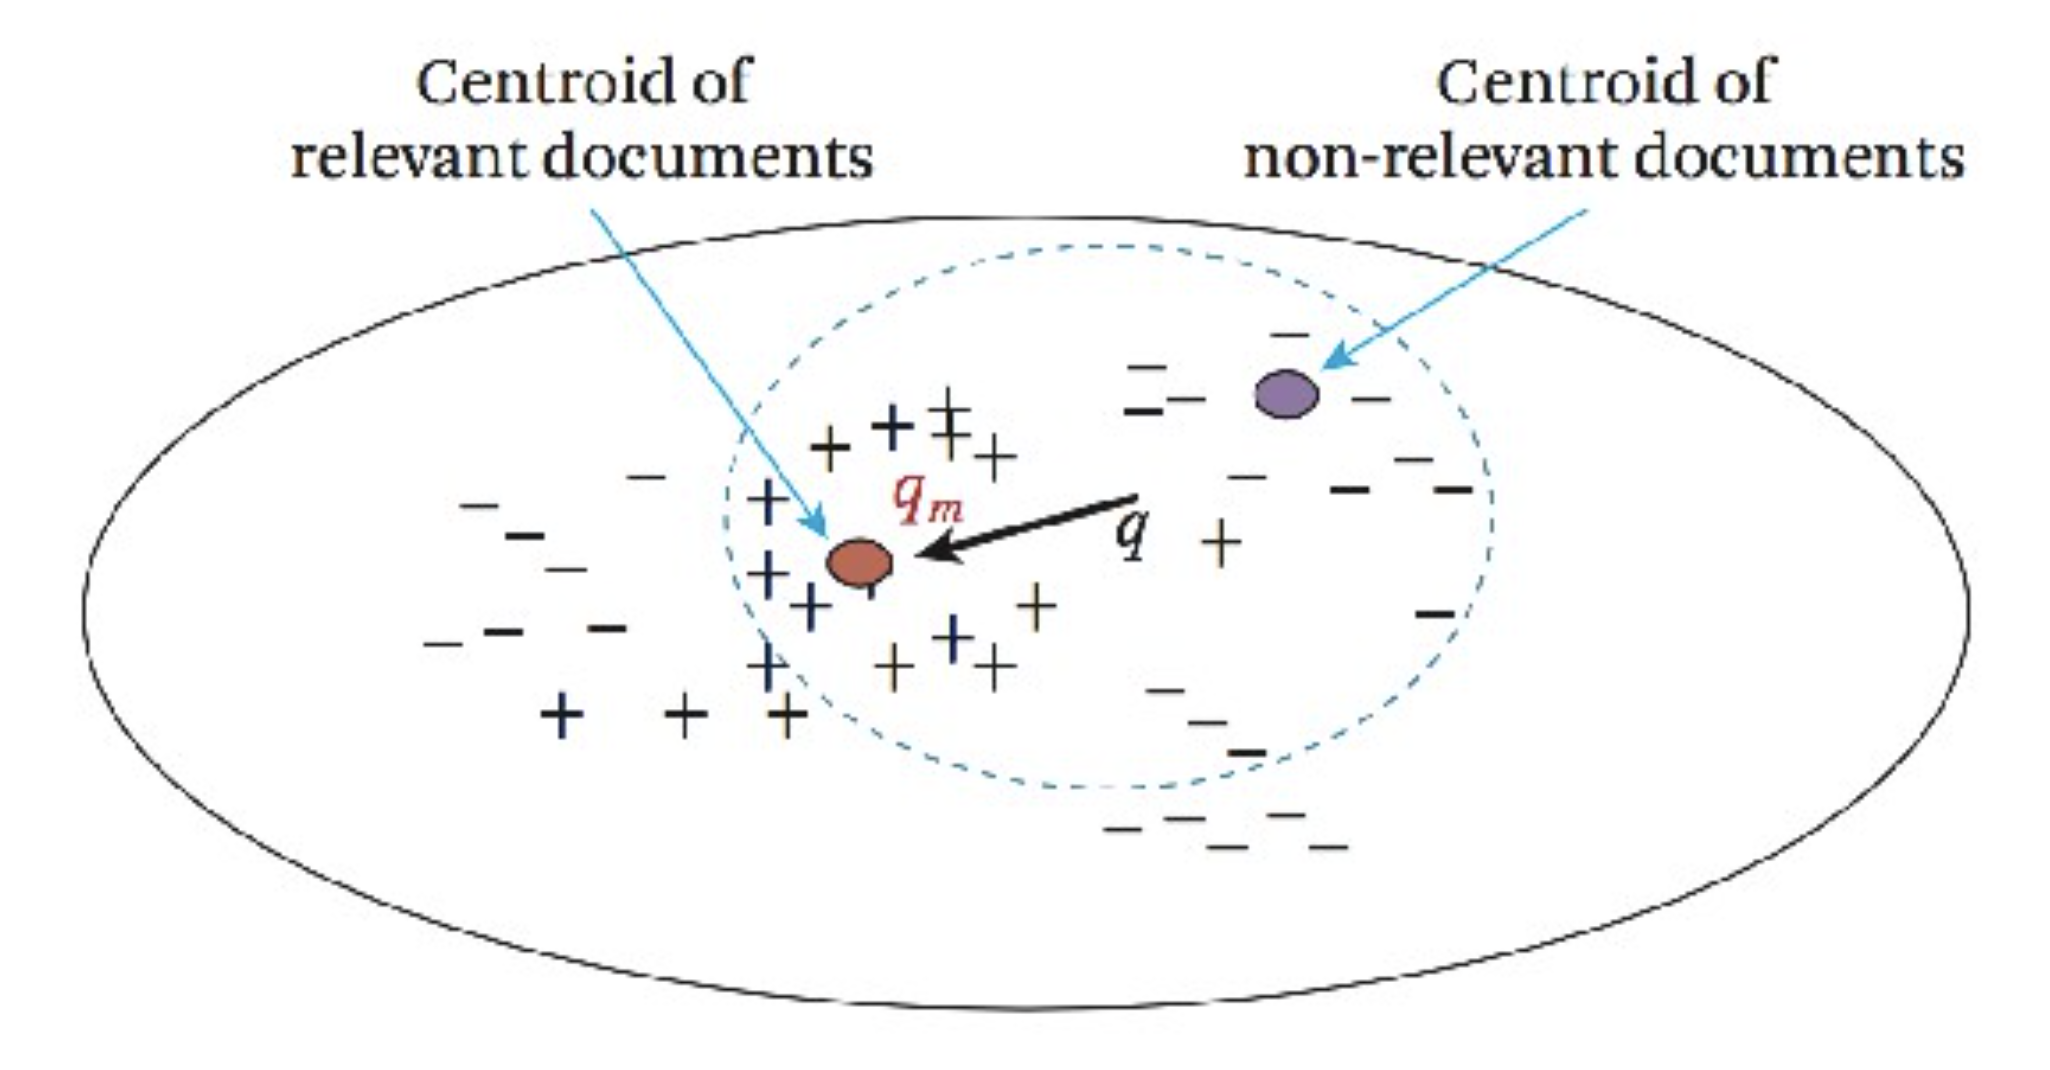
\includegraphics[width=9cm]{rocchio.png}
\end{center}
The Rocchio algorithm was invented in 1971 and revolves around the concept of an \textbf{optimal query}. The optimal query maximises the difference between the average vector representing the relevant documents and the average vector representing the non-relevant documents. \\ \\
The modified query results in a longer expanded query. This is because the terms that occur frequently in the relevant documents will be added to the modified query and those that occur frequently in non-relevant documents will be removed. \\ \\
The Rocchio feedback formula is the following:
\[ q'_j = \alpha \cdot q_j + \beta \cdot \frac{1}{|R|} \cdot \sum_{D_i \in R} d_{ij} - \gamma \cdot \frac{1}{|NR|} \cdot \sum_{D_i \in NR} d_{ij} \]
Where $\alpha$ is a constant of value 8, $\beta$ is a constant of value 16, $\gamma$ is a constant of value 4, \textit{R} is the group of relevant documents -- $|R|$ is the size of that group, and \textit{NR} is the group of non-relevant groups -- $|NR|$ is the size of that group.

\section{System Evaluation}
Evaluation is concerned with assessing if the system carries out its tasks properly. This is the key to building an effective and efficient search engine. \\ \\
In an evaluation assessment, three measurements are checked:

\begin{itemize}
	\item \textbf{Efficiency}
	\vspace{.2cm} \\
	It measures if the information retrieval system carries out its tasks with an optimal use of its resources.
	
	\item \textbf{Effectiveness}
	\vspace{.2cm} \\
	It measures if the information retrieval system finds what the user wants to find.
	
	\item \textbf{Usability}
	\vspace{.2cm} \\
	It measures how useful is the system for real user tasks.
\end{itemize}
Furthermore, these measurements are usually carried out in a controlled laboratory environment.

\subsection{The Cranfield Evaluation Methodology}
This is the primary approach to an evaluation of an information retrieval system's effectiveness. The main idea of this test is to build reusable test collections and to define measures of effectiveness. In order to do this, we need:

\begin{itemize}
	\item A sample collection of documents;
	\item A sample collection of queries/topics;
	\item Relevance judgements;
	\item Measures to quantify how well a system's result matches the ideal ranked list.
\end{itemize}

\subsection{TREC}
TREC (Text REtrieval Conference) is an evaluation forum that started in 1992 in order to encourage research in information retrieval evaluation and to compare information retrieval systems.

\subsection{Effectiveness}
The two main measurements to evaluate effectiveness in an information retrieval system are \textbf{precision} and \textbf{recall}. \\ \\
\textbf{Precision} is a measurement in which we simply compute to what extent all the retrieval results are relevant. On the other hand, \textbf{recall} measures the completeness of coverage of relevant documents in the retrieval system.

\subsubsection{Classification Errors}
There are two main classification error in information retrieval systems, these are:

\begin{itemize}
	\item \textbf{False Positive - Type I Error}
	\vspace{.2cm} \\
	It is the ratio of non-relevant documents that have been retrieved.
	
	\item \textbf{False Negative - Type II Error}
	\vspace{.2cm} \\
	It is the ratio of the relevant documents that have not been retrieved.
\end{itemize}

\subsubsection{F1 Score}
The F1 score is the harmonic mean of recall and precision. Its formula is the following:
\[ F = \frac{1}{\frac{1}{2} \left( \frac{1}{R} + \frac{1}{P} \right)} = \frac{2RP}{R+P} \] \\
Where $R$ is the recall and $P$ is the precision of the information retrieval system.

\subsection{Computing the Performance of a System}
\subsubsection{Mean Average Precision}
In order to properly compute the performance of a system we need to analyse several queries. To compute the average precision for each query, and to summarize the rankings from multiple queries, we use the \textbf{Mean Average Precision (MAP)}. \\ \\
The MAP measurement assumes that the user is interested in finding many relevant documents for each query. This requires many relevance judgements in the text collection. \\ \\
In order to obtain the MAP, first we compute the average precision of each query, and then we compute the mean of these means.

\subsubsection{Interpolation of Recall-Precision Graphs}
In order to better understand a recall-precision graph, we use the following formula:

\[ P(R) = \max \{ P' : R' \geq R \wedge (R', P') \in S \} \] \\
Where \textit{S} is the set of observed $(R, P)$ points. This formula defines the precision at any recall level as the maximum precision observed in any point in \textit{S} at a higher recall level. This will produce a step function that is both easier to understand and compare than the original, and allows us to define precision when the $R = 0$. \\

\begin{figure}[!htb]
	\begin{minipage}{0.48\textwidth}
	 	\centering
	 	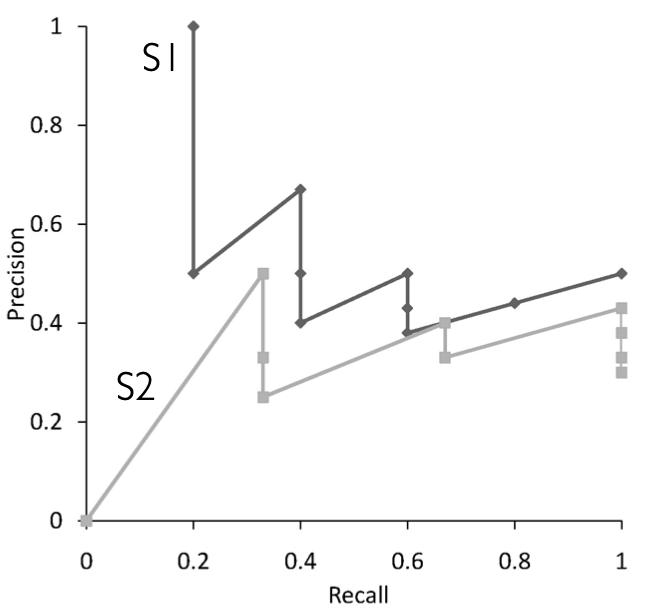
\includegraphics[width=.9\linewidth]{rpg.png}
   	\end{minipage}\hfill
   	\begin{minipage}{0.48\textwidth}
     		\centering
     		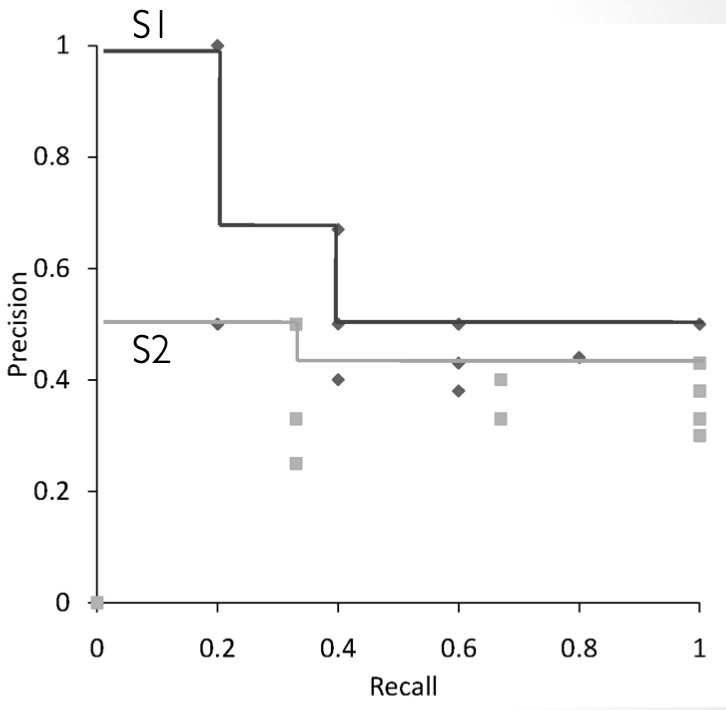
\includegraphics[width=.9\linewidth]{interpolation.png}
   	\end{minipage}
\end{figure}
\noindent Here the figure on the \textit{left} represents the original recall-precision graph, while the one on the \textit{right} represents the image on the left after we apply interpolation.

\section{User Evaluation}
In user evaluation, we test the user interaction in addition to the quality of the information retrieval system. The quality of the interface of the search engine cannot be tested without the user involvement. \\ \\
In this evaluation we have a low volume of queries and artificial tasks -- meaning that the user carries out the search, but in an artificial situation.

\subsection{Experimental Design}
This is an experimental evaluation, thus it needs to:

\begin{enumerate}
	\item \textbf{Decide the aim of the evaluation}
	\vspace{.2cm} \\
	We need to decide which are the features that we need to evaluate, and what is the goal of this new feature.	
	
	\item \textbf{Formulate experimental hypotheses}
	\vspace{.2cm}\\
	The aims of the experiment need to be expressed as experimental hypotheses to be tested. These hypotheses also tell us some of the information we will need to gather.
	
	\item \textbf{Define an experimental methodology}
	\vspace{.2cm} \\
	We need to gather:
	
	\begin{itemize}
		\item \textbf{Collections}
		\vspace{.2cm} \\
		What are we searching?
		
		\item \textbf{People}
		\vspace{.2cm} \\
		Who does the searching?
		
		\item \textbf{Systems}
		\vspace{.2cm} \\
		Usually either two or more systems or two or more versions of the same machines are compared.
		
		\item \textbf{Search Tasks}
		\vspace{.2cm} \\
		Search tasks can be given or can be real. In order to test the user on these tasks, we use an \textbf{experimental matrix} -- for example a Latin Square Design. Tasks can also be: decision tasks, background knowledge or fact search.
	\end{itemize}
	
	\item \textbf{Define criteria for data comparison}
	\vspace{.2cm} \\
	While quantitative data can be easy to compare, qualitative data is more difficult to compare. In order to compare the latter kind of data, we can use a Likert scale.
	
	\item \textbf{Perform experiments}
	\vspace{.2cm} \\
	Try not to introduce any bias in the experiment, this could alter the results and make the whole output of the experiment unusable.
		
	\item \textbf{Analyse the obtained data}
	\vspace{.2cm} \\
	Use proper methods of statistical data analysis on quantitative data.
\end{enumerate}

\subsection{Qualitative and Quantitative Data}
\textbf{Quantitative data} measures the search effectiveness. On the other hand, \textbf{qualitative data} measures the user's perception of a system. Qualitative data is assessed by using tests for statistical significance, such as: Mann-Whitney test, T-test, Chi-squared tests...

\subsection{Operational Evaluation}
It is similar to user evaluation, but in this case it deals with real users in real search situations and with real tasks on a real collection. \\ \\
This is an expensive and difficult-to-run test, but it is a very good test of the system in a real situation.

\section{Web Search Engine}
A web search engine is divided into three main parts: crawling, indexing and ranking.

\subsection{Web Crawling}
Find and download pages automatically. The web provides for the collection, which is way too big and constantly growing. \\ \\
A \textbf{web crawler} is a software that crawls web pages and puts them into cache. The following is the process of crawling.

\begin{enumerate}
	\item Connect to a DNS server
	\item The DNS server translates the hostname into an IP address
	\item There is an attempt from the scraper to connect to the host using a specific port
	\item A \verb|GET| request is sent to the web server
\end{enumerate}

\subsubsection{Focused Crawling}
Here the crawler attempt to download only the pages that are about a specific topic. This method relies on the fact that pages about a topic tend to have links to other pages on the same topic. \\ \\
The crawler uses a \textbf{text classifier} in order to determine whether a page is on topic.

\subsubsection{Deep Web}
The 96\% of available websites are in the deep web. These websites can be divided into three main groups:

\begin{itemize}
	\item \textbf{Private websites}
	\vspace{.2cm} \\
	These are websites that might require the user to login, or simply websites that do not have incoming links.
	
	\item \textbf{Form Results}
	\vspace{.2cm} \\
	These are websites that can be reached only after entering some data inside of a form.
	
	\item \textbf{Scripted Pages}
	\vspace{.2cm} \\
	These are pages that use client-side programming languages to generate links.
\end{itemize}

\subsubsection{Politeness Policies}
In order not to flood web servers with thousands of requests all at the same time, politeness policies are used by web crawlers. These are, for example:

\begin{itemize}
	\item Limiting the number of requests per second
	\item Respecting the \verb|robots.txt| file of the website
\end{itemize}

\subsection{Ranking Algorithms}
Ranking algorithms are used in order to find which websites are the most authoritative and generally better. One way of performing such ranking is by using the famous PageRank algorithm. \\ \\
PageRank is used to compute the "popularity" of the given webpages. It does so by considering the websites' inlinks. \\ \\
The \textbf{Random Surfer Model} is the basic concept behind PageRank. I uses the following algorithm:

\begin{enumerate}
	\item Choose a random number $r$ between 0 and 1
	\item If $r < \alpha$, then go to a random page
	\item If $r \geq \alpha$, then click a link at random on the current page
	\item Start again from the beginning
\end{enumerate}
More generally, PageRank is defined by the following formula:

\[ PR(u) = \frac{\lambda}{N} + (1 - \lambda) \cdot \sum_{v \in B_v} \frac{PR(v)}{L_v} \]
Where $B_v$ is the set of pages that point to $u$, $L_v$ is the number of outgoing links from page $v$, $N$ is the number of pages, and $\lambda$ is a constant which is typically set to $0.15$. \\ \\
Interesting pages detected by the algorithm fall into two classes:

\begin{itemize}
	\item \textbf{Authorities}
	\vspace{.2cm} \\
	These are pages that contain useful information. In practice, these pages have many incoming links.
	
	\item \textbf{Hubs}
	\vspace{.2cm} \\
	These are pages that list a number of authorities. In practice, these pages have many outgoing links to different authorities.
\end{itemize}
Authorities are ranked based on the sum of the votes that each Hub has, while the Hubs are ranked based on the sum of votes of the Authorities they are pointing to.

\section{Recommender Systems}
\textbf{Information filtering} deals with dynamic collections, and generates long and elaborated profiles and filters. It also serves long term information needs. On the other hand, \textbf{information retrieval} deals with static collections. In this case it server short-lived queries. \\ \\
Another comparison is between \textbf{information filtering} and \textbf{routing}. While \textbf{information filtering} chooses documents to show based on a binary decision. \textbf{routing} relies on ranking in order to determine the best results. In the first case, we have the problem of documents being too much or too few. \\ \\
There are three different types of information filtering:

\begin{itemize}
	\item Content-based information filtering
	\item Collaborative/Social information filtering
	\item Use-base information filtering
\end{itemize}

\subsection{Content-Based Information Filtering}
This types of filtering makes decisions for individual users based on what the system learned the user likes or dislikes. Interest and preferences are inferred based on previous user feedback. \\ \\
Some of the downsides of these techniques are:

\begin{itemize}
	\item The filtering decision is binary
	\item The initialization phase is based only on the profile text or very few initial examples
	\item There is a limited relevance judgement ("yes" documents)
\end{itemize}

\subsection{Collaborative Filtering}
In this case the filtering decisions for an individual user are based on the judgements of other users. Interest and preference are inferred from that of other similar users. \\ \\
This kind of filtering is based in user profile comparison, thus cannot work with only one user. \\ \\
Furthermore, collaborative filtering will make several assumptions, such as:

\begin{itemize}
	\item Users with the same interests will have the same preferences
	\item Users with the same preferences will likely have the same interests
	\item A sufficiently large number of users preferences is available
\end{itemize}
Some possible improvements are:

\begin{itemize}
	\item Dealing with missing values by setting defaults
	\item Using Inverse User Frequency
\end{itemize}
Some problems, instead, are:

\begin{itemize}
	\item The size of the data needs to be very big
	\item There is a problem known as Cold Start. This happens when new documents cannot be recommended because there are no previous references
\end{itemize}

\subsection{Use-Based Information Filtering}
This method identifies which documents are semantically relevant to a user profile by inferring relevance from user behaviour. \\ \\
Some problems with this method are:

\begin{itemize}
	\item User profiles can be messy
	\item It can be very intrusive and not respect the user's right to privacy
\end{itemize}

\section{Text Clustering}
Text clustering is used in order to group similar objects together by discovering their natural structure. \\ \\
In order to assess similarity between objects, the user must define the perspective -- i.e. a bias.

\subsection{Clustering in Text Retrieval}
Clusters can be created based on \textit{concepts}, \textit{topics} or \textit{themes}. It can be divided into two main categories:

\begin{itemize}
	\item \textbf{Similarity-Based Clustering}
	\vspace{.2cm} \\
	Which can be either \textit{agglomerative} or \textit{divisive}.
	
	\item \textbf{Model-Based Clustering}
	\vspace{.2cm} \\
	Data is assumed to have been generated from a finite mixture of component models.
\end{itemize}
This is an unsupervised method of grouping objects together.

\subsubsection{Similarity-Based Clustering}
In order to perform similarity-based clustering, we need to:

\begin{itemize}
	\item Provide a clustering bias
	\item Find the optimal partitioning in order to maximize intra-group similarity, and at the same time minimize inter-group similarity
\end{itemize}
In order to obtain the optimal clusterings, we need to follow this algorithm:

\begin{enumerate}
	\item Progressively construct a hierarchy of clusters using one of the following two methods:
	
	\begin{itemize}
		\item \textbf{Agglomerative Method}
		\vspace{.2cm} \\
		Gradually group similar objects into larger clusters.
			
		\item \textbf{Divisive Method}
		\vspace{.2cm} \\
		Gradually partition the data into smaller clusters.
	\end{itemize}
	
	\item Start with an initial tentative clustering and iteratively improve it
\end{enumerate}

\subsubsection{Agglomerative Hierarchical Clustering}
The algorithm for this type of clustering method is the following:

\begin{enumerate}
	\item Assume a similarity function
	\item Gradually group objects in a bottom-up fashion in order to form a group hierarchy
	\item Stop whenever some stopping criterion is met
\end{enumerate}

\subsection{Clustering Strategies}
Several clustering strategies exist, these are:

\begin{itemize}
	\item \textbf{Single-Linkage}
	\vspace{.2cm} \\
	It creates loose clusters and is based on individual decisions, thus being sensitive to outliers. The clustering cost of this strategy is defined by the following formula:
	\[ Cost = \min\{~d(x_i, x_j)~|~x_i \in C_i, x_j \in C_j~\} \]
	Where $d(x_i, x_j)$ is the distance between the two elements, and $C$ is a cluster.
	
	\item \textbf{Complete-Linkage}
	\vspace{.2cm} \\
	It creates tight clusters and is based on individual decisions, thus being sensitive to outliers. The clustering cost of this strategy is defined by the following formula:
	\[ Cost = \max\{~d(x_i, x_j)~|~x_i \in C_i, x_j \in C_j~\} \]
	Where $d(x_i, x_j)$ is the distance between the two elements, and $C$ is a cluster.
	
	\item \textbf{Average-Linkage}
	\vspace{.2cm} \\
	It creates clusters in between the two clusters above and is based on group decisions, thus not being sensitive to outliers. The clustering cost of this strategy is defined by the following formula:
	\[ Cost = \frac{\sum_{x_i \in C_i, x_j \in C_j} d(x_i, x_j)}{|C_i| ~ |C_j|} \]
	Where $d(x_i, x_j)$ is the distance between the two elements, and $C$ is a cluster.
\end{itemize}

\subsection{Cluster Representative}
In order to represent a cluster of many points, we use something called a \textbf{clustroid}, which is a point that is closer to all other points. \\ \\
A \textbf{centroid}, instead, is the average of all data points in a cluster. This means that it is an artificial point -- that can correspond to a real point in the cluster. \\ \\
The following is a graphical representation of a cluster:

\begin{center}
	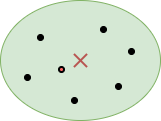
\includegraphics[width=3cm]{./clustering.png}
\end{center}
Where the \textit{cluster} is the green oval, the red x is the \textit{centroid}, the black dot is a regular \textit{data point}, and the black dot with the red dot inside it is a \textit{clustroid}. \\ \\
"Closer to" -- relative to data points -- can be defined in several different ways:

\begin{itemize}
	\item The smallest maximum distance to other points
	\item The smallest average distance to other points
	\item The smallest sum of squares of distance to other points
\end{itemize}
The "nearness" of clusters, on the other hand, can be determined using several different approaches:

\begin{itemize}
	\item Treat the clustroids as if they were centroids and measure the distance between the two clusters
	\item Use the \textbf{intercluster distance} by involving the minimum of the distances between any two points -- one from each cluster
	\item Use the \textbf{cohesion of clusters} notion by involving the maximum distance of the cluster to another cluster's clustroid. After doing so, merge the clusters whose union is the most cohesive
\end{itemize}

\subsection{K-Means Clustering}
In order to initialize this method, we do the following:

\begin{itemize}
	\item Assume that we are working in an Euclidean space
	\item Pick a value for the number of clusters, $k$
	\item Initialise the clusters by picking one point per cluster
\end{itemize}
After having initialized the clusters we can proceed to populate them:

\begin{enumerate}
	\item For each point, place it in the cluster whose current centroid is the nearest
	\item After all points have been assigned, update the locations of the centroids
	\item Reassign all points to their closest centroid
	\item Repeat steps 2 and 3 until convergence, meaning that the points do not move any more between clusters
\end{enumerate}

\subsection{Clustering Evaluation}
The evaluation of clustering aims at maximizing the following aspects:

\begin{itemize}
	\item \textbf{Coherence}
	\vspace{.2cm} \\
	How similar objects in the same cluster are.
	
	\item \textbf{Separation}
	\vspace{.2cm} \\
	How far away objects in different clusters are.
	
	\item \textbf{Utility}
	\vspace{.2cm} \\
	How useful the discovered clusters are for an application.
\end{itemize}
In order to perform a good evaluation of clusterings, we need to proceed as follows:

\begin{enumerate}
	\item Given a predefined test set, have humans create an ideal clustering result
	\item Use a system to produce clusters from the same test set
	\item Quantify the similarity between the two clusterings
\end{enumerate}

\section{Text Categorization}
In text categorization object are put into classes -- or categories. \\ \\
Given a set of predefined categories and a training set of labelled text objects, the task is to classify a text object int one or more of the categories. \\ \\
Categories can be of two different types:

\begin{itemize}
	\item \textbf{Internal}
	\vspace{.2cm} \\
	They characterize a text object.
	
	\item \textbf{External}
	\vspace{.2cm} \\
	They characterize an entity associated with the text object.
\end{itemize}

\subsection{Manual Categorization Method}
In this case the category of an object is determined based on rules carefully designed to reflect domain knowledge about the problem. \\ \\
This method is labour intensive, and does not scale up well. It's also not robust, this is because it can't handle uncertainties in rules.

\subsection{Automatic Categorization Methods}
Manual categorization method limitations can be fixed with the use of machine learning. \\ \\
Machine learning is used in order to learn \textit{soft} rules for categorization based on training data. All of the methods rely in discriminative features of text objects in order to distinguish categories. Moreover, they also adjust the weights on features in order to minimize errors.

\subsection{Generative Classifiers}
In this case the algorithm learn what the data looks like in each category. In order to model the classifiers, we can use the Bayes Rule.

\subsection{Discriminative Classifiers}
In this case the algorithm learns what features separate each category. \\ \\
In order to do so, we can use the Support Vector Machine or the k-Nearest Neighbors.

\subsection{Feature Selection}
A feature is an attribute of an object that we wish to classify. \\ \\
Feature selection methods reduce the number of features by only choosing the most useful.

\subsection{Information Gain}
This is a commonly used feature selection measure based on information theory. The model is trained with the top $k$ best features -- with $k$ usually being a small number.

\subsection{Naïve Bayes Classifier}
This is a typical example of a \textbf{generative classifier}. It is a probabilistic model based on Bayes' Rule. The formula of this model is:

\[ P(C~|~D) = \frac{P(D~|~C) \cdot P(C)}{\sum_{c \in C}P(D~|~C=c) \cdot P(C=c)} \] \\
Where $C$ is a random variable corresponding to the class, and $D$ is a random variable corresponding to the input -- for an example document. \\ \\
Documents are classified according to the following formula:

\begin{align*}
Class(d) & = \arg \max_{c \in C} P(c~|~d) \\
& = \arg \max_{c \in C} \frac{p(d~|~c) \cdot P(c)}{\sum_{c \in C} P(d~|~c) \cdot P(c)}
\end{align*}
Where $P(d~|~c)$ is the probability that document $d$ is observed given the class $c$, and $P(c)$ is the probability of observing class $c$.

\subsubsection{Estimating P(c)}
This term is estimated as the proportion of training documents in class $c$. The formula for this is:

\[ P(c) = \frac{N_c}{N} \] \\
Where $N_c$ is the number of training documents in class $c$, and $N$ is the total number of training documents.

\subsubsection{Estimating P(d $|$ c)}
This term is estimated depending on the event space used to represent the documents. The event space is the set of all possible outcomes for a given random variable.

\subsubsection{Multiple Bernoulli Event Space}
This is a natural way of modelling distributions over binary vectors -- which indicate whether a term is present or not inside of a document. The formula for this event space is the following:

\[ f(k;p) = p^k(1-p)^{1-k} \] \\
On the other hand, if we want to check the frequency of a term in a document, we would have to use \textbf{multinomial distribution}.

\subsubsection{Multinomial Distribution}
By using this distribution, the way $P(d~|~c)$ is computed changes, In this case we would have:

\[ P(d~|~c) \propto \prod_{w \in v} P(w~|~c)^{tf_{w,d}} \] \\
Where $P(w~|~c)$ can be either a \textbf{Laplacian Smoothed (Jelinek-Mercer) Estimate}, which formula is the following:

\[ P(w~|~c) = \frac{tf_{w,c} + 1}{|c| + |V|} \] \\
Or a \textbf{Collection Smoothed (Diricklet) Estimate}, which formula is the following:

\[ P(w~|~c) = \frac{tf_{w,c} + \mu \frac{cfw}{|c|}}{|c| + \mu} \]

\subsection{Support Vector Machine}
This is an example of a discriminative model based on geometrical principles. \\ \\
The goal here is to, given a set of inputs labelled $+$ and $-$, find the best hyperplane that separates these two groups. \\ \\
A hyperplane is a generalization of a line to higher dimensions. It is defined by the vector $w$. The best hyperplane -- in this case -- is the one with the maximum margin between the two classes. This margin can be computed by using the following formula:

\[ Margin(w) = \frac{|w \cdot x^{-}| + |w \cdot w^{+}|}{||w||} \] \\ 
It is generally assumed that $ |w \cdot x^{-}| + |w \cdot w^{+}| = 1 $. Thus, in order to find the largest margin, we must maximize the following:

\[ Margin(w) = \frac{2}{||w||} \]

\subsubsection{The Kernel Trick}
Since data cannot always be linearly-separable, we can transform it in order to make it linearly-separable. Computing vector math in very high dimensional spaces is costly. \\ \\
For this reasons we use something known are the kernel trick. It basically allows for very high-dimensional dot products to be computed efficiently.

\subsubsection{Non-Binary Classification with SVMs}
There are two ways to do it:

\begin{itemize}
	\item \textbf{One Versus All}
	\vspace{.2cm} \\
	Train the model as a "class $c$ versus not class $c$" SVM for every class. If there are $k$ classes, $k$ classifiers must be trained. The items are classified based on the following formula:
	\[ Class(x) = \arg \max_c w_c \cdot x \]
	
	\item \textbf{One Versus One}
	\vspace{.2cm} \\
	A binary classifier is trained for every pair of classes, Thus
	\[ k \frac{k-1}{2} \]\\
	Classifiers must be trained. This method is computationally expensive for large values of $k$.
\end{itemize}

\subsection{K-Nearest Neighbors}
The goal of this algorithm is to find $k$ examples in the training set that are the most similar to the text object to be classified, by performing a search for every testing instance. \\ \\
After this has been done, we assign the category that is most common in these neighbor text objects.

\subsection{Classifier Evaluation}
In order to evaluate classifiers, we can use one of the following metrics:

\begin{itemize}
	\item Accuracy
	\item Precision
	\item Recall
	\item F-Measure
	\item ROC Curve Analysis
\end{itemize}

\section{Opinion Mining}
Opinions are extremely important in order for us to make decisions. The problems with mining opinions may be several, such as:

\begin{itemize}
	\item There are subtle ways of expressing opinions
	\item Opinions could be written in a non-standard or incorrect English
	\item There could be instances of opinion reversals
\end{itemize}
\textbf{Fake News} is false or misleading information presented in a way to damage the reputation of a person or entity. These fake news can generate misled opinions.

\subsection{Opinion Analysis}
An opinion is a subjective statement describing what a person believes or thinks about something. \\ \\
An opinion is a quintuple defined as:

\[ O = (e_i, a_{ij}, oo_{ijkl}, h_k, t_l) \] \\
Where $e_i$ is the name of an entity, $a_{ij}$ is an aspect of $e_i$, $oo_{ijkl}$ is the orientation of the point about aspect $a_{ij}$ of $e_i$, $h_k$ is the opinion holder, and $t_l$ is the date and time when the opinion is expressed by $h_k$.

\subsection{Levels of Opinion Analysis}
There are three levels of opinion analysis:

\begin{itemize}
	\item \textbf{Document Level}
	\vspace{.2cm} \\
	Classify the whole document as expressing a positive or negative sentiment.
	
	\item \textbf{Sentence Level}
	\vspace{.2cm} \\
	Determines whether each sentence expresses a positive, negative or neutral opinion.
	
	\item \textbf{Aspect Level}
	\vspace{.2cm} \\
	It performs finer-grained analysis and determines the sentiments towards different aspects.
\end{itemize}

\subsection{Sentiment Lexicons}
Sentiment lexicons are lists of words and expressions used in order to express people's subjective feelings and sentiments/opinions. \\ \\
In order to build such lexicons, we can use one of the following:

\begin{itemize}
	\item Manual lexicons
	\item Dictionary-based lexicons
	\item Corpus-based lexicons
\end{itemize}
The advantages of these methods are the following:

\begin{itemize}
	\item They are fairly accurate independently of the medium
	\item There is no need for a training corpus
	\item They are easily extendible to other domains only with the insertion of additional affective words
	\item It is easy to rationalize the prediction output
\end{itemize}
On the other hand, the disadvantages of these methods are the following:

\begin{itemize}
	\item They are costly to implement
	\item The typically underperform compared to well-trained, in-domain ML models
	\item They are sensitive to affective dictionary coverage
\end{itemize}

\subsection{Sentiment Analysis Approaches}
There are three main sentiment analysis approaches:

\begin{itemize}
	\item \textbf{Unsupervised}
	\vspace{.2cm} \\
	Such as \textit{NlP patterns} and \textit{lexicons}.
	
	\item \textbf{Supervised}
	\vspace{.2cm} \\
	Such as \textit{SVMs} and \textit{Naïve Bayes}.
	
	\item \textbf{Semi-Supervised}
	\vspace{.2cm} \\
	Such as a \textit{lexicon} + a \textit{classifier}.
\end{itemize}

\subsubsection{Unsupervised Approaches}
Here no training of the data is required. These approaches are also known as \textbf{lexicon-based approaches}. \\ \\
These approaches rely on external lexical resources that associate a popularity score to each term. The sentiment of the term depends on the sentiment of document depends on the sentiment of the terms which compose it.
\subsubsection{Supervised Approaches}
Here the "learn by example" paradigm is put into practice. A machine learning algorithm is provided with lots of examples. \\ \\
The algorithm is used to extract characteristic patterns for each category and build a predictive model.

\subsubsection{Semi-Supervised Approach}
The following are the steps to follow in order to use a semi-supervised approach:

\begin{enumerate}
	\item Get manually annotated documents from the domain of interest
	\item Train any standard classifier using a \textit{bag-of=words} as feature
	\item Apply the trained classifier to a test corpus or an application
\end{enumerate}
The main advantage of this method is that it tends to attain a good predictive accuracy. \\ \\
The disadvantages of this method are:

\begin{itemize}
	\item The need for a very specific training corpus
	\item Domain sensitivity
\end{itemize}

\subsection{Opinion Retrieval}
Opinion retrieval is the retrieval of documents that are about a topic, and that express an opinion about that topic. \\ \\
The steps of opinion retrieval are the following:

\begin{enumerate}
	\item Rank documents based on topical relevance -- by using TF*IDF ranking schemes, language modelling approaches...
	\item The results obtained are re-ranked or filtered by applying one or more heuristics for detecting opinions. Most approaches use a liner combination of relevance score and opinion score in order to rank documents. The formula for it is the following:
	\[ Score(Q,D) = (1 - \alpha) \cdot rel(Q,D^{+}) + \alpha \cdot op(Q,D) \]
	Where $rel$ is the relevance feedback score and $op$ is the opinion score.
\end{enumerate}

\section{Audio Indexing and Retrieval}
Audio is a signal whose frequencies range is in the human audible range. \\ \\
Audio is normally displayed as a waveform, and has several physical characteristics that can be used to describe it. \\ \\
From the physical characteristics of the waveform we can derive a number of acoustic features, such as:

\begin{itemize}
	\item \textbf{Pitch}
	\vspace{.2cm} \\
	Greatest common divisor of peak in a Fourier spectra.
	
	\item \textbf{Brightness}
	\vspace{.2cm} \\
	Centroid of short-time Fourier magnitude spectra.
	
	\item \textbf{Loudness}
	\vspace{.2cm} \\
	Root-mean square of the audio signal -- measured in decibels.
	
	\item \textbf{Bandwidth}
	\vspace{.2cm} \\
	Magnitude-weighted average of the difference between the spectral components and the centroid.
	
	\item \textbf{Harmonicity}
	\vspace{,2cm} \\
	Deviation of the sound's spectrum from a harmonic spectrum.
\end{itemize}

\subsection{Acoustic Features}
these features are represented as functions changing over time. In order to sample these acoustic features, we can follow the following algorithm:

\begin{enumerate}
	\item Compute the acoustic features at a certain time interval
	\item Derive the average value $\mu$, the variance $\sigma$, and the autocorrection $\rho$ for each feature
	\item Weight the features value by amplitude
\end{enumerate}

\subsection{Content-Based Audio Retrieval}
If audio has been indexed as a series of feature vectors, such as:

\[ s = ((\mu l, \sigma l, \rho l), ..., (\mu h, \sigma h, \rho h)) \] \\
Then the retrieval process can be carried out by comparing the feature vectors using a mathematical model.

\section{Speech Indexing and Retrieval}
In this case the indexing is concerned with capturing the semantics of what is being said, rather than the sound. In order to index such documents there are several approaches:

\begin{itemize}
	\item Controlled vocabulary indexing
	\item Ranked retrieval based on associated text
	\item Social filtering based on user's rating
	\item Automatic feature=based speech indexing
\end{itemize}
Some speech features could be:

\begin{itemize}
	\item Identity
	\item Language
	\item Content
\end{itemize}

\subsection{Speech Recognition Systems}
Speech recognition systems are basically black boxes that transform voice into text. \\ \\
Some problems with speech recognition are:

\begin{itemize}
	\item Word boundaries
	\item Adjacent phonemes influencing one another
	\item The same phoneme cannot be repeated twice without changing its physical representation due to different acoustic conditions
	\item Ambiguity in the phonetic to orthographic transcription
	\item Words that are out of the vocabulary
\end{itemize}

\subsection{Spoken Document Retrieval}
In order to create a spoken document retrieval model, we need a large vocabulary word recognition where transcripts of spoken documents are created. Some other possible approaches are:

\begin{itemize}
	\item Using subword units
	\item Recognizing only a small set of keywords
\end{itemize}

\subsubsection{LVSR Approach}
Its main goal is to transform a SDR into a textual IR. Thus spoken documents should be converted into text, and then retrieved using classic textual retrieval techniques.

\subsubsection{Subwords Units Approach}
In this case syllable sequences are used as indexing features. the user query is then decomposed into indexing features and the best matches are retrieved. \\ \\
Phoneme sequences can be also used as indexing features.

\subsubsection{Word Spotting Approach}
A small set of keywords can be used as indexing features. In the indexing process keyword spotting is carried out, and documents are retrieved based in the presence of a combination of keywords. \\ \\
This approach can be very useful for topic identification and spotting, though it is disappearing as a result of speech recognition getting faster and better.

\section{Image Indexing and Retrieval}
In order to retrieve images, there are three main approaches:

\begin{itemize}
	\item Keyword based approach
	\item Based on visual properties of the image
	\item Concept based approach
\end{itemize}

\subsection{Keyword Based Approach}
Here images are annotated using keywords. This can be expensive since images should be manually annotated. \\ \\
Manual annotation is also prone to subjectivity, and low level visual properties are almost impossible for a human to capture and index. \\ \\
Since -- in this case -- image description is textual, we could use standard IR techniques in order to retrieve the images.

\subsection{Visually Based Approach}
This approach is usually referred to as \textbf{Content-Based Image Retrieval} (CBIR). The similarity between the query and the documents is computed by comparing visual features, such as:

\begin{itemize}
	\item Color
	\item Texture
	\item Shape
\end{itemize}
Images -- like in the case of audio -- can be represented by using a set of feature vectors. These are described as:

\[ If_i = (If_{i1}, ..., If_{in}) \] \\
While queries are represented as:

\[ Qf_i = (Qf_{i1}, ..., Qf_{in}) \] \\
As we can see, here we have a form of \textit{query-by-example}.

\subsubsection{Feature Vector}
Each feature has its own representation, and provide a \textit{synthetic} view of a certain feature. \\ \\
One image characteristic may be represented by many features.

\subsubsection{Color Based Retrieval}
A very simple approach is to:

\begin{enumerate}
	\item Represent an image as a rectangular pixel raster
	\item Represent each pixel as a quantified color
	\item Cont the number of pixels in each color bin
	\item Compute a vector similarity
\end{enumerate}
A \textbf{color histogram} can be generated from images. The problem with comparing images by color is that sometimes two images that represent the same concept could have very different color histograms.

\subsubsection{Blobworld Segmentation}
A complex query formulation is often based on the selection of some visual features. The blobs are used to help the system match two images that are similar with each other.

\subsection{Concept-Based Approach}
The system is able to capture the most important points of an image. Based on these points, the system can then check is other images have these same points or not. \\ \\
A downside to this approach is that the knowledge of the application domain is required.

\section{Video Indexing and Retrieval}
A video, before being indexed and retrieved, needs to be segmented. The following are the possible segmentations of a video:

\begin{itemize}
 \item \textbf{Scene}
 \vspace{.2cm} \\
 This is a collection of semantically related \textit{shots}.
 
 \item \textbf{Shot}
 \vspace{.2cm} \\
 This is a sequence of \textit{frames} recorded in one camera operation.
 
 \item \textbf{Frames}
 \vspace{.2cm} \\
 The series of images that compose the video.
\end{itemize}

\subsection{Shot Boundary Detection}
Shot boundary detection is very computationally expensive and not that precise. \\ \\
A simple way to detect shot boundaries is represented by the following algorithm:

\begin{enumerate}
	\item Get two frames
	\item Create a color histogram for each of the frames
	\item Concatenate the color histogram in order to form a color signature for each frame
	\item Using the cosine similarity measure, check if the frames are similar or not
\end{enumerate}

\subsection{Non-Sequential Browsing}
A visual inspection of the video enables fora much better retrieval process. This is also known as \textbf{video browsing}. \\ \\
Since browsing frames sequentially is time consuming, then a solution would be to structure a video in terms of shots and scenes. These structures are known as \textbf{scene trees}.

\subsection{Content-Based Indexing}
In order to perform a proper retrieval, we need to combine different detector, such as:

\begin{itemize}
	\item Text features
	\item Visual features
	\item Audio/Voice features
\end{itemize}
The best solution is to combine all features together, matching the domain and characteristics of the images.

\end{document}
